\documentclass[11pt,letterpaper]{article}

\usepackage[margin=1in]{geometry}
\usepackage{amsmath, amssymb}
\usepackage{booktabs}
\usepackage{graphicx}
\usepackage{hyperref}
\usepackage{caption}
\usepackage{microtype}
\usepackage{parskip}
\usepackage{enumitem}

\setlist{itemsep=2pt, topsep=2pt, parsep=0pt}
\setlength{\parskip}{4pt plus 1pt minus 1pt}
\captionsetup{font=small, labelfont=bf, skip=4pt}

\graphicspath{{../plots/}{plots/}}
\hypersetup{colorlinks=true, linkcolor=blue, urlcolor=blue, citecolor=blue}

\title{\vspace{-2em}CME 213 Final Project\\
\large Building and Profiling a Small GPT-2 Training Pipeline in CUDA and MPI}
\author{Nils Astrup Toft \and Sondre Rogde}
\date{June 8, 2026}

\begin{document}
\maketitle\vspace{-1.5em}

\begin{abstract}
We build a GPT-2-style transformer training pipeline from scratch in C++/CUDA with
MPI data parallelism. Every operation in the forward and backward pass is implemented
as a custom CUDA kernel, and we profile each against the hardware roofline using
Nsight Compute and Nsight Systems. Register tiling lifts GEMM from 13.5\% to 58.6\%
of FP32 peak; float4 vectorized loads bring memory-bandwidth-bound kernels to 64--70\%
of peak bandwidth. Pre-allocating backward scratch buffers and fusing 50 per-tensor
\texttt{MPI\_Allreduce} calls into one together reduce 4-GPU step time from 74.5\,ms
to 59.8\,ms, raising strong-scaling efficiency from 55\% to 62\% at $P=4$.
\end{abstract}

\section{Project Description}

We train a decoder-only GPT-2-style transformer on sequences of token IDs. The input
is a batch of integer token sequences of shape $(B, S)$; the output is vocabulary
logit distributions of shape $(B, S, V)$, from which we compute a cross-entropy loss
and backpropagate gradients to update all model parameters with Adam.
The model uses Pre-LayerNorm transformer blocks: each block applies
multi-head self-attention followed by a two-layer feed-forward network (FFN),
both with residual connections. We denote $B$ = batch size, $S$ = sequence length,
$C$ = model dimension, $H$ = attention heads, $D = C/H$ = head dimension,
$V$ = vocabulary size.

\paragraph{Why it is hard.}
The forward pass is dominated by dense matrix multiplications. A single forward
step for a 6-layer model at $C=256$ already involves 36+ GEMMs. Self-attention
scales quadratically with $S$ in naive implementations. Multi-GPU training
matters because batch sizes large enough for stable convergence easily exceed
single-GPU memory, and per-step time on a single GPU multiplies up to hours
for larger models.

\paragraph{Scope.}
We train a model with $n_\text{layers}=6$, $C=256$, $H=16$, $S=128$, $V=512$,
giving approximately 5\,M parameters. Experiments use both synthetic data
(for scaling and profiling reproducibility) and Wikitext-2 (to confirm
real training dynamics). We also build a text-generation inference binary.
The focus is profiling and optimization analysis, not convergence.

\section{Algorithms and State of the Art}

\paragraph{GEMM.}
Dense matrix multiplication dominates transformer FLOPs. The state of the art is
cuBLAS~\cite{cublas}, which reaches 70--80\% of FP32 peak on large matrices by
combining shared-memory tiling, register-file accumulation, and tensor cores
(on Ampere+). We implement the shared-memory tiled variant from Boehm~\cite{boehm2022}
and extend it with $8 \times 8$ register tiling, targeting ~60\% of cuBLAS.

\paragraph{Flash Attention.}
Standard attention materializes the $S \times S$ score matrix, using $O(S^2)$
memory. Flash Attention~\cite{dao2022} tiles over $S$ in SRAM and maintains
an online softmax, reducing memory to $O(S \cdot D)$ while computing the exact
same result. We implement the Flash Attention 1 forward pass; the backward
uses the standard $O(S^2)$ realization.

\paragraph{The full transformer.}
We implement Pre-LayerNorm transformer blocks as in GPT-2~\cite{radford2019},
with Adam~\cite{kingma2015} as the optimizer.
GPT-2 was originally released in four sizes (117M to 1.5B parameters);
our 5M-parameter model is much smaller and is designed for profiling, not for
competitive language modeling.

\paragraph{Data-parallel distributed training.}
The standard approach is to replicate the model on each rank, have each rank
compute gradients on a local mini-batch, and synchronize via all-reduce before
the optimizer step. Horovod~\cite{sergeev2018} and PyTorch DDP fuse gradient
tensors into large buffers before calling \texttt{MPI\_Allreduce} (or NCCL)
to amortize per-call startup latency. Karpathy's \texttt{llm.c}~\cite{karpathy2024}
follows the same idea in pure C. We implement the same fusing strategy from scratch.

\section{Parallelization Strategy}

\paragraph{System overview.}
The implementation has five layers: CUDA kernels, stateful layer modules,
a \texttt{GPT2} model class, a \texttt{Trainer} orchestrating
forward/backward/Adam, and an MPI wrapper for data parallelism. All tensors
are FP32 row-major; hidden states are $(B \cdot S, C)$.

\paragraph{GEMM kernels.}
We implement three GEMM variants ($C = AB$, $C = AB^T$, $C = A^T B$), each
using a $128 \times 128$ output tile loaded into shared memory with a $BK=8$
strip across $K$. Each $8 \times 8$ thread block computes a $8 \times 8$
register sub-tile (64 FP32 accumulators per thread). Loads from global memory
are coalesced: adjacent threads access adjacent elements. The inner $k$-loop
is \texttt{\#pragma unroll} to eliminate branch overhead and expose 64
independent FMAs per shared-memory load.

\paragraph{Flash Attention forward.}
The kernel tiles $Q$, $K$, $V$ into SRAM. For each query tile it streams over
key/value tiles, maintaining a running max $m^{(j)}$ and normalization $\ell^{(j)}$
with an online correction factor $e^{m^{(j-1)}-m^{(j)}}$ when the tile max rises.
Causal masking is applied per tile by zeroing scores where the key position exceeds
the query position. One thread block handles one $(B, H)$ query tile.

\paragraph{Bandwidth-bound kernels.}
LayerNorm uses a two-pass warp reduction to avoid catastrophic cancellation.
GELU, Softmax, and Cross-Entropy use \texttt{float4} 128-bit vectorized loads
so each thread moves 4 floats per instruction, cutting the load instruction
count by $4 \times$ versus scalar loads.

\paragraph{MPI data parallelism.}
Each MPI rank initializes on one GPU. Rank 0 broadcasts initial weights with
\texttt{MPI\_Bcast}. Each training step:
(i) every rank takes its contiguous slice of the global batch using a shared
step-based seed;
(ii) forward and backward on the local slice;
(iii) \texttt{allreduce\_gradients} averages all gradient tensors;
(iv) Adam update on each rank using the averaged gradient, keeping weights
synchronized without further communication.

The \textbf{fused allreduce} packs all gradient tensors into one
\texttt{cudaMallocHost} pinned buffer (D$\to$H per tensor), issues a single
\texttt{MPI\_Allreduce(MPI\_SUM)}, then scatters back (H$\to$D). Pinned memory
lets the DMA engine transfer at full PCIe bandwidth.

\section{Performance Model}

\paragraph{Roofline for GEMM.}
The hardware ceilings are 16.31\,TFLOPS FP32 and 672\,GB/s bandwidth
(RTX\,6000, sm\_75), giving a ridge point of $\approx$24\,FLOP/byte.
For the basic tiled kernel (one output per thread), the effective arithmetic
intensity is $T/4 = 8$\,FLOP/byte -- below the ridge, so the kernel is
memory-bound in shared memory. With $8 \times 8$ register tiling, the
intensity rises to $8 \times 8 = 64$\,FLOP/byte, comfortably above the ridge.
The roofline prediction is that register tiling moves GEMM from memory-bound
to compute-bound.

\paragraph{Communication cost.}
For \texttt{MPI\_Allreduce} with message size $n$ bytes we model
$T(n) = \alpha + n/b_\text{eff}$, where $\alpha$ is startup latency and
$b_\text{eff}$ is the effective all-reduce bandwidth. For our 5M-parameter
model, the total gradient is $\approx$20\,MB. The allreduce benchmark
(Figure~\ref{fig:comm}) fits $\alpha \approx 2$--$6\,\mu$s per call
(same-node shared-memory transport) and $b_\text{eff} \approx 3$\,GB/s.
With 50 per-tensor calls, the startup cost is only $50 \times 6 = 300\,\mu$s.
Fusing all calls into one is therefore unlikely to save much time on this
single-node setup. In contrast, the bandwidth cost for 20\,MB at 3\,GB/s
is $\approx$7\,ms, and PCIe D$\to$H$\to$D transfers for the same data cost an
additional $\approx$8\,ms -- the dominant overhead not visible from the $\alpha$
model alone.

\paragraph{Amdahl and isoefficiency.}
For strong scaling, parallel efficiency is $E(P) = T_1/(P \cdot T_P)$.
The serial fraction is $f = (1/E_P - 1)/(P - 1/E_P)$.
For 90\% isoefficiency, compute time per rank must satisfy
$T_\text{compute} \geq T_\text{comm}/0.1$, i.e., at least $10\times$ the
communication time.

\section{Benchmarking and Instrumentation}

\paragraph{Nsight Compute (kernel level).}
We run \texttt{ncu --set full} to capture hardware counters: achieved TFLOPS
and GB/s, SM occupancy, L1/L2 hit rates, and roofline coordinates for every
kernel in a single forward+backward pass. We profile both a before and an
after snapshot (see \texttt{profiles/ncu\_kernels\_before.ncu-rep} and
\texttt{profiles/ncu\_kernels\_after.ncu-rep}) to separate the contribution
of each optimization.

\paragraph{Nsight Systems (system level).}
We annotate the training loop with NVTX markers (\texttt{forward\_backward},
\texttt{allreduce}, \texttt{optimizer}). \texttt{nsys} captures the full CUDA
+ MPI + OS timeline. The $\approx$30\,ms/step overhead from per-step
\texttt{cudaMalloc} calls -- invisible in coarse \texttt{std::chrono} timing --
was found this way.

\paragraph{Scaling and allreduce benchmarks.}
Per-step wall time is measured with \texttt{std::chrono::steady\_clock} on
rank 0; allreduce is timed separately. We collect 20-step averages.
The standalone \texttt{allreduce\_bench} binary runs 100 trials of
\texttt{MPI\_Allreduce} at each message size from 256 bytes to 64\,MB
to fit $\alpha + \beta n$ for $P = 2$ and $P = 4$.

\section{Bottleneck Analysis}

Nsight Compute and Nsight Systems together identify four distinct bottlenecks
in the unoptimized implementation:

\textbf{(1) GEMM below the ridge point.}
The basic tiled GEMM achieves 2.20\,TFLOPS = 13.5\% of FP32 peak. With one
output element per thread and tile size $T=32$, the arithmetic intensity is only
8\,FLOP/byte -- the kernel is memory-bound in shared memory, not global memory.
Each thread reads shared-memory tiles without accumulating enough FMAs per read
to saturate the FP32 units.

\textbf{(2) Scalar loads for memory-bandwidth-bound ops.}
LayerNorm, GELU, Softmax, and Cross-Entropy have $O(1)$\,FLOP/byte arithmetic
intensity; they are firmly memory-bound. Before optimization, GELU achieved
only $\approx$17\% of peak bandwidth because scalar 32-bit loads underutilize
the 128-bit memory bus, issuing 4$\times$ more load instructions than needed.

\textbf{(3) Per-tensor allreduce calls.}
With 50 separate \texttt{MPI\_Allreduce} calls per step, each call incurs
startup overhead -- even at only $\alpha \approx 6\,\mu$s on shared-memory
transport. More importantly, 50 separate D$\to$H and H$\to$D \texttt{cudaMemcpy}
calls each have their own driver overhead, adding up to $\sim$3\,ms above the
fused-call baseline.

\textbf{(4) Per-step cudaMalloc in the backward path.}
\texttt{MultiHeadAttention::backward()} allocated 11 device buffers on every
call, including two $B \times H \times S \times S$ attention score matrices
($\approx$4\,MB each at training config). \texttt{cudaMalloc} is a synchronizing
call that flushes the GPU command queue. At training config with $B=16$, this
caused $\approx$30\,ms of blocking overhead per step, visible as large spikes
in the Nsight Systems timeline.

\section{Algorithmic Variants and Their Effect on Performance}

\paragraph{Variant 1: Register tiling for GEMM.}
We replace the 1-output-per-thread tiled kernel with an 8$\times$8 register-tiled
version (64 FP32 accumulators per thread). The roofline prediction -- that this
would move GEMM from memory-bound to compute-bound -- is confirmed: throughput
jumps from 2.20\,TFLOPS (13.5\% peak) to \textbf{9.56\,TFLOPS (58.6\% peak)},
roughly 4.3$\times$ improvement. cuBLAS achieves approximately 70--80\% of peak
on Turing, so our register-tiled kernel reaches $\sim$75\% of cuBLAS performance.
Figure~\ref{fig:roofline} shows both GEMM points on the roofline.

\paragraph{Variant 2: Float4 vectorized loads for memory-bound kernels.}
We replace scalar 32-bit loads in GELU, Softmax, Cross-Entropy, and LayerNorm
with \texttt{float4} 128-bit loads. Each thread now moves 4 floats per instruction.
As shown in Table~\ref{tab:kernels}, the optimized kernels reach 430--470\,GB/s
(64--70\% of the 672\,GB/s peak), versus $\approx$17\% before vectorization
for GELU -- a $\approx$4$\times$ bandwidth improvement. The bottleneck shifts
from instruction-count to raw PCIe/HBM bandwidth.

\paragraph{Variant 3: Fused gradient allreduce.}
We compare 50 individual \texttt{MPI\_Allreduce} calls against one call on a
single packed pinned buffer. The communication volume is identical.
As predicted by the $\alpha+\beta n$ model, the startup-latency saving is small
on a single node ($50\alpha \approx 300\,\mu$s) -- but removing 50 separate
\texttt{cudaMemcpy} call pairs reduces comm time from 18.6\,ms to 15.6\,ms
($\approx$3\,ms saving). The residual 15.6\,ms is bandwidth-dominated PCIe
transfer. The remaining gap to the theoretical bandwidth bound
(Figure~\ref{fig:comm}) represents the D$\to$H$\to$D round trip -- recoverable
only with CUDA-aware MPI.

\paragraph{Variant 4: Pre-allocated backward scratch.}
We move all 11 per-step device buffer allocations in \texttt{MultiHeadAttention}
and 7 more in \texttt{TransformerBlock} to constructor time. Step time at 1 rank
drops from \textbf{162.7\,ms to 148.8\,ms} ($\approx$14\,ms saving), isolating
the \texttt{cudaMalloc} overhead. Combined with the fused allreduce, 4-rank step
time drops from 74.5\,ms to 59.8\,ms.

\section{Scalability Analysis}

Table~\ref{tab:scaling} reports strong and weak scaling results; the corresponding
efficiency curves are in Figure~\ref{fig:scaling}.

\begin{table}[h]
  \centering\small\setlength{\tabcolsep}{5pt}
  \begin{tabular}{@{}llrrrrrr@{}}
    \toprule
    \textbf{Config} & \textbf{Sweep} & $P$ &
    \textbf{step (ms)} & \textbf{comm (ms)} & \textbf{comm\%} &
    \textbf{speedup} & \textbf{eff.} \\
    \midrule
    Before opt. & strong & 1 & 162.7 & 0.0  & ---   & $1.00\times$ & 100\% \\
    Before opt. & strong & 2 & 105.1 & 17.7 & 16.8  & $1.55\times$ & 77\%  \\
    Before opt. & strong & 4 &  74.5 & 18.6 & 25.0  & $2.19\times$ & 55\%  \\
    \midrule
    After opt.  & strong & 1 & 148.8 & 0.0  & ---   & $1.00\times$ & 100\% \\
    After opt.  & strong & 2 &  92.5 & 14.4 & 15.6  & $1.61\times$ & 80\%  \\
    After opt.  & strong & 4 &  59.8 & 15.6 & 26.1  & $2.49\times$ & 62\%  \\
    \midrule
    After opt.  & weak   & 1 &  43.6 & 0.0  & ---   & ---          & 100\% \\
    After opt.  & weak   & 2 &  57.9 & 14.3 & 24.6  & ---          & 75\%  \\
    After opt.  & weak   & 4 &  59.8 & 15.6 & 26.1  & ---          & 73\%  \\
    \bottomrule
  \end{tabular}
  \caption{Scaling results on a single 4-GPU node (RTX\,6000, sm\_75).
    Strong: total $B=16$. Weak: local $B=4$ per rank. $n_\text{layers}=6$,
    $C=256$, $S=128$. 20-step averages.}
  \label{tab:scaling}
\end{table}

\begin{figure}[h]
  \centering
  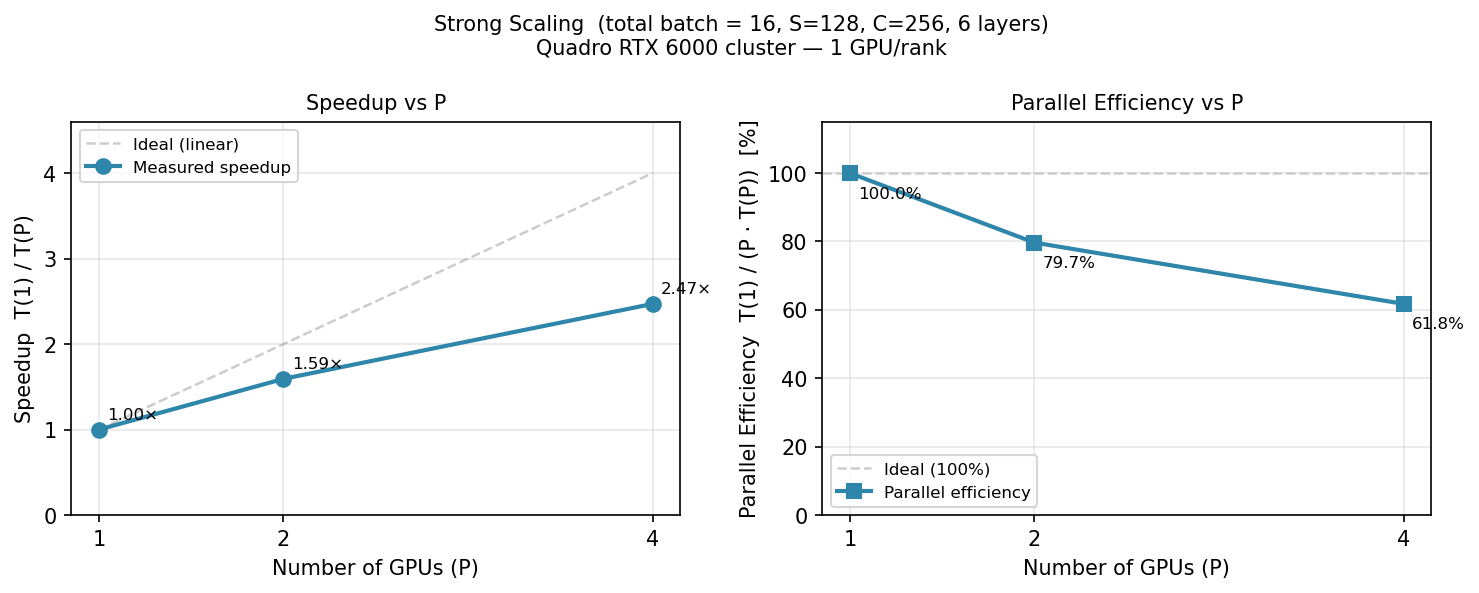
\includegraphics[width=0.95\linewidth]{strong_scaling}
  \caption{Strong scaling: step time breakdown and parallel efficiency for
    $P = 1, 2, 4$. Total $B=16$, 20-step averages on node hpcc-gpu-5-1.
    \emph{Before} is the unoptimized baseline; \emph{After} includes all four
    optimization variants. Comm = \texttt{allreduce\_gradients} time.}
  \label{fig:scaling}
\end{figure}

\paragraph{Amdahl analysis.}
At $P=4$ the strong-scaling efficiency is $E_4 = 62\%$. The Amdahl serial
fraction is
\[
  f = \frac{1/E_4 - 1}{P - 1/E_4}
    = \frac{1/0.62 - 1}{4 - 1/0.62} \approx 0.25.
\]
This 25\% serial fraction is almost entirely communication: the comm fraction
at $P=4$ is 26\% of step time (Table~\ref{tab:scaling}).

\paragraph{Isoefficiency.}
For 90\% efficiency we need $T_\text{compute} \geq 10 \times T_\text{comm}$.
Our current $P=4$ compute time is $\approx$44\,ms and comm is 15.6\,ms,
giving a ratio of 2.8 -- well below the threshold. To reach 90\% efficiency
at $P=4$, we would need to increase compute by $\approx$3.5$\times$
(e.g., local batch size 14 instead of 4), or more practically,
use CUDA-aware MPI to cut comm to $\sim$7\,ms (the allreduce-only time),
which would raise the ratio to $\approx$6.3.

\paragraph{Weak scaling.}
Weak efficiency drops from 100\% (P=1) to 75\% (P=2) and 73\% (P=4), mainly
because communication time grows at the same rate regardless of the increase
in compute work. The comm fraction at $P=4$ in weak scaling (26\%) is nearly
identical to strong scaling -- confirming that communication cost is essentially
fixed by gradient size, not batch size.

\section{Correctness and Verification}

Each kernel is validated independently. The test suite (\texttt{tests/}) compares
GPU output to a CPU reference using a combined criterion: relative error $\leq 10^{-3}$
or absolute error $\leq 10^{-5}$ (the absolute guard handles near-zero values
that would spike relative error). Forward kernels are additionally compared to
PyTorch-generated \texttt{.bin} reference tensors. All forward and backward tests
pass on the cluster: GEMM (sizes $32^3$ to $4096^3$), LayerNorm (forward and
backward), GELU, Softmax, Cross-Entropy, Flash Attention forward, and the naive
attention backward.

Multi-rank correctness is confirmed in three ways.
First, the step-1 loss is bit-identical across $P = 1, 2, 4$ (loss = 6.5336),
confirming that \texttt{MPI\_Bcast} and the deterministic forward pass are correct.
Second, all configurations drive the loss toward the random-token entropy floor
over 20 steps, and the model trains correctly on Wikitext-2 (loss falls from
9.27 at step 1 to below 6.0 by step 300 with 4 ranks).
Third, at \texttt{ranks=4, local\_B=4}, the strong and weak step times agree
within 0.02\,ms, confirming correct batch decomposition.

\section{Discussion, Limitations, and Future Work}

\paragraph{What gave the biggest payoff.}
Pre-allocating backward scratch and fusing the allreduce together saved
$\approx$14\,ms per step at $P=4$ -- nearly 20\% of total step time.
Neither bottleneck was visible in coarse \texttt{chrono} timing; both required
Nsight Systems to find. Register tiling required more implementation effort
and improved GEMM throughput by 4.3$\times$, but GEMM is only one of many
kernels so the absolute step-time saving is smaller.
Float4 vectorization was a quick win that brought memory-bound kernels to
64--70\% of bandwidth peak with a few lines of code.

\paragraph{Limitations.}
We do not use CUDA-aware MPI. The host-staged D$\to$H$\to$D copies add
$\approx$8\,ms per step (the gap between allreduce benchmark time and measured
comm time), which CUDA-aware MPI over NVLink would eliminate. The Flash
Attention backward is $O(S^2)$; the recomputation-based backward from
Flash Attention 2~\cite{dao2023} would be needed to scale to longer sequences.
BF16 is not implemented: on Turing (sm\_75), BF16 runs on regular CUDA cores
at FP32 throughput, so there is no compute benefit. On Ampere and Hopper,
native BF16 tensor cores give $4 \times$ throughput.

\paragraph{What we would do differently.}
Pre-allocating backward scratch from the start would have saved hours of
debugging. Starting with a bucketed allreduce (as Horovod does) rather than
a per-tensor loop would also have been the right default. Looking ahead, the
obvious next steps are CUDA-aware MPI (removes PCIe overhead), batched GEMM
for the attention backward (eliminates remaining per-head dispatch loops),
and BF16 on newer hardware.

\begin{thebibliography}{9}

\bibitem{radford2019}
A.\ Radford et al.
Language Models are Unsupervised Multitask Learners.
OpenAI Technical Report, 2019.

\bibitem{dao2022}
T.\ Dao, D.\ Fu, S.\ Ermon, A.\ Rudra, and C.\ R\'{e}.
FlashAttention: Fast and Memory-Efficient Exact Attention with IO-Awareness.
In \textit{NeurIPS}, 2022.

\bibitem{dao2023}
T.\ Dao.
FlashAttention-2: Faster Attention with Better Parallelism.
\textit{arXiv:2307.08691}, 2023.

\bibitem{boehm2022}
S.\ Boehm.
How to Optimize a CUDA Matmul Kernel for cuBLAS-like Performance.
\textit{siboehm.com}, 2022.

\bibitem{cublas}
NVIDIA. cuBLAS Library User Guide. NVIDIA Developer Documentation, 2024.

\bibitem{sergeev2018}
A.\ Sergeev and M.\ Del Balso.
Horovod: Fast and Easy Distributed Deep Learning in TensorFlow.
\textit{arXiv:1802.05799}, 2018.

\bibitem{karpathy2024}
A.\ Karpathy. \texttt{llm.c}.
\url{https://github.com/karpathy/llm.c}, 2024.

\bibitem{kingma2015}
D.\ Kingma and J.\ Ba.
Adam: A Method for Stochastic Optimization.
In \textit{ICLR}, 2015.

\bibitem{williams2009}
S.\ Williams, A.\ Waterman, and D.\ Patterson.
Roofline: An Insightful Visual Performance Model.
\textit{CACM}, 52(4):65--76, 2009.

\end{thebibliography}

\appendix

\section{Kernel Performance Details}
\label{app:kernels}

\begin{table}[h]
  \centering\small\setlength{\tabcolsep}{5pt}
  \begin{tabular}{@{}llrrrr@{}}
    \toprule
    \textbf{Kernel} & \textbf{Bound} &
    \textbf{Baseline} & \textbf{\% peak} &
    \textbf{Optimized} & \textbf{\% peak} \\
    \midrule
    GEMM ($4096^3$)         & Compute & 2.20\,TFLOPS & 13.5\% & 9.56\,TFLOPS & 58.6\% \\
    Flash Attn ($B=1$, $S=2048$) & Compute & ---      & ---    & 2.09\,TFLOPS & 12.8\% \\
    LayerNorm ($N=8192$)    & BW      & $\approx$110\,GB/s & 16\% & 432\,GB/s & 64\% \\
    GELU ($N=4$M)           & BW      & $\approx$114\,GB/s & 17\% & 471\,GB/s & 70\% \\
    Softmax ($V=30000$)     & BW      & ---          & ---    & 431\,GB/s    & 64\% \\
    Cross-Entropy ($V=30000$) & BW    & ---          & ---    & 472\,GB/s    & 70\% \\
    \bottomrule
  \end{tabular}
  \caption{Per-kernel performance: baseline vs.\ optimized on RTX\,6000 (sm\_75).
    Peak: 16.31\,TFLOPS FP32, 672\,GB/s bandwidth.
    Baseline BW numbers for GELU/LayerNorm are from Nsight Compute before
    float4 vectorization; ``---'' means the kernel was not in the before profile.}
  \label{tab:kernels}
\end{table}

\begin{figure}[h]
  \centering
  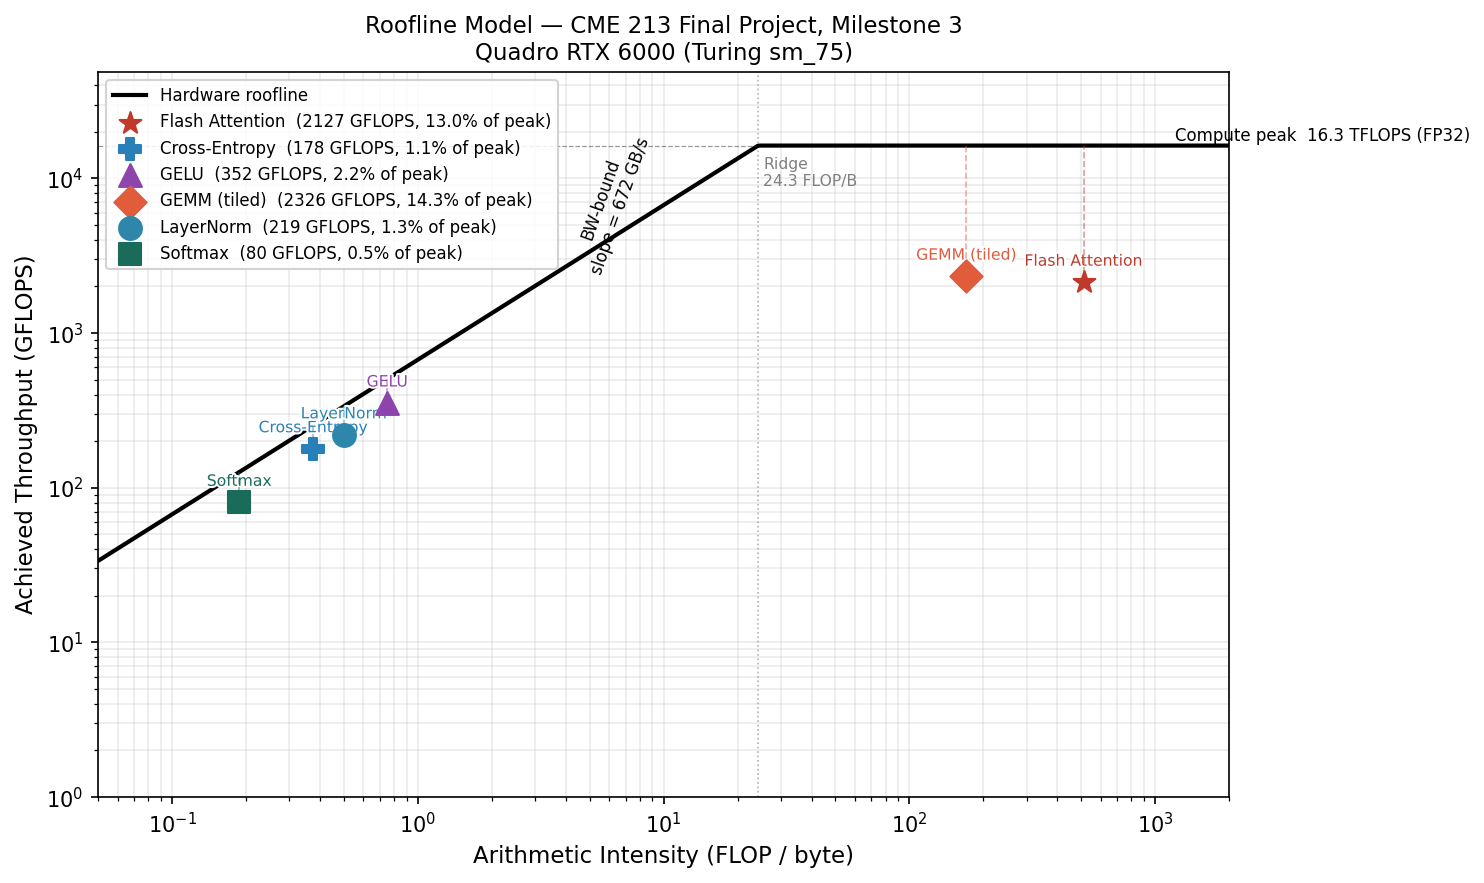
\includegraphics[width=0.92\linewidth]{roofline}
  \caption{Roofline model for RTX\,6000 (sm\_75). FP32 ceiling: 16.31\,TFLOPS;
    bandwidth ceiling: 672\,GB/s; ridge: $\approx$24\,FLOP/byte.
    Both GEMM points (before/after register tiling) and bandwidth-bound kernels
    (after float4 vectorization) are shown.}
  \label{fig:roofline}
\end{figure}

\section{Communication Benchmark}
\label{app:comm}

\begin{figure}[h]
  \centering
  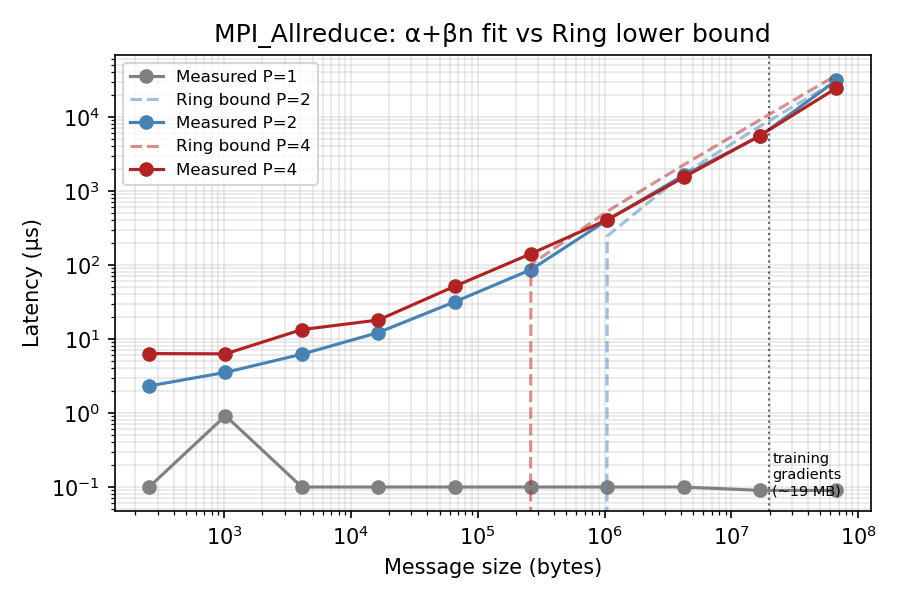
\includegraphics[width=0.88\linewidth]{comm_alpha_beta}
  \caption{\texttt{MPI\_Allreduce} latency vs.\ message size for $P=2$ and $P=4$,
    100-trial averages. The dashed line is the theoretical Ring lower bound
    $T_\text{ring} = 2(P-1)/P\,(\alpha + n/b)$.
    At large sizes both curves are bandwidth-dominated at $\approx$3\,GB/s
    effective throughput (PCIe D$\to$H$\to$D round trip).
    CUDA-aware MPI would bypass these copies and approach the NVLink bandwidth.}
  \label{fig:comm}
\end{figure}

\section{Weak Scaling}
\label{app:weak}

\begin{figure}[h]
  \centering
  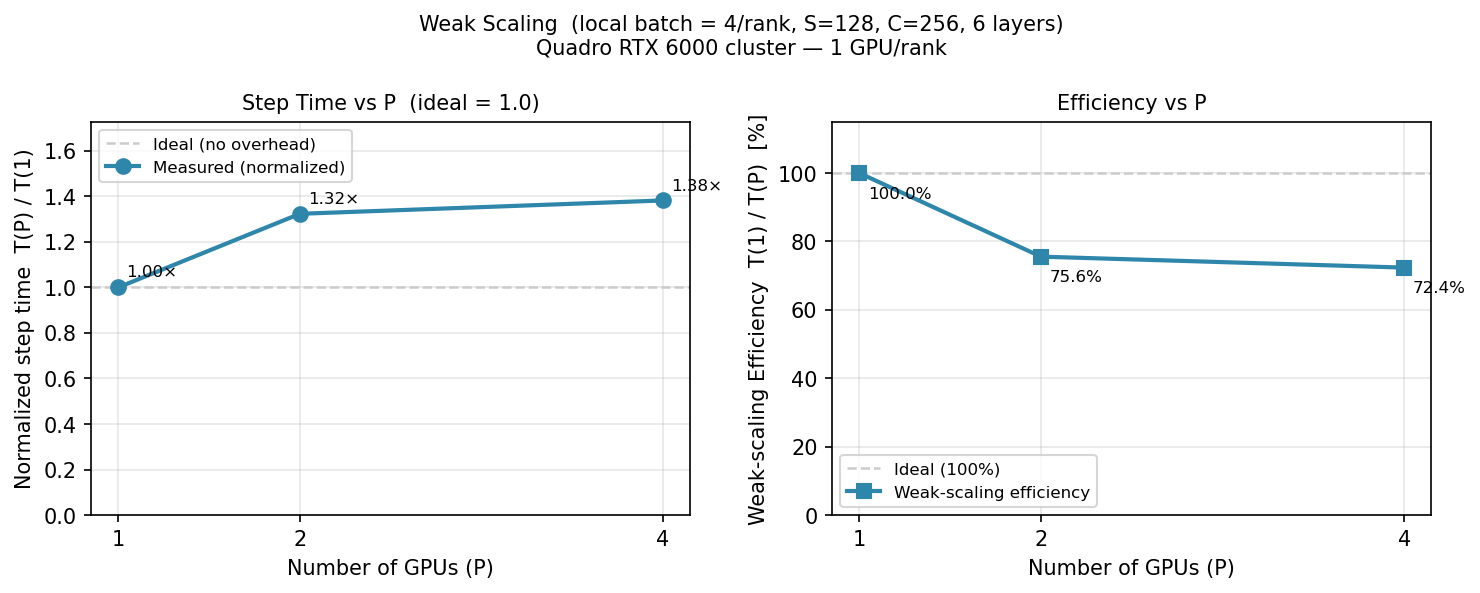
\includegraphics[width=0.88\linewidth]{weak_scaling}
  \caption{Weak scaling efficiency (local $B=4$ per rank). Efficiency at $P=4$
    drops to 73\%, driven by a nearly fixed communication cost ($\approx$15.6\,ms)
    regardless of batch size -- confirming that comm is dominated by gradient size,
    not compute volume.}
  \label{fig:weak}
\end{figure}

\end{document}
